\documentclass[../masterarbeit.tex]{subfiles}
\begin{document}
	



\subsection{Feature selection}

It is a challenging and significant task in the field of data science to create machine learning models from high dimensional data sets. Machine learning research has assumed that too many columns of data lead to a reduction in prediction quality. This phenomenon is caused by the fact that the algorithm recognizes non-existent patterns in the data set due to the amount of features and creates its learning file based on this. These non-existent patterns are learned by the model because it tries to interpret the noise in the data or irrelevant information when the data set is too complex. So the model tries to fit too much to the training data and end up overfitting, wich means it gets good results with the train data, but has a high error on test data. \autocite[]{ibm-overfitting:2022} \\
The opposite can happen if there are too much important features removed from the dataset in terms of the feature selection. In this case the model underfits and it gets an high training error as well as an high test error. \autocite[]{ibm-overfitting:2022}
Both overfitting and underfitting lead to a bad performance quality of the machine learning model and it is a challenging task to find the optimum between them \textcite[]{SUBASI202091}. The three different variants overfitting, underfitting and the optimum way a model can fit the data is visualized in figure 1. The line drawn through the data points shows how accurately the model has been fitted to the data set. So you can see that in the first visualization, only a straight line was drawn and lots of the points ended up on the wrong side of the line. In the last oft the three figures, which represents overfitting, the line is snaked so that every outliner also is on the right class. In this case the points that are closer to the other class than to their corresponding one are also correctly classified. With such a fitting it is difficult to correctly classify unseen data in border areas. The center illustration shows the optimal case that classifies many points correctly, but makes no exceptions for outliers. \\
\begin{figure}[h]
    \centering
    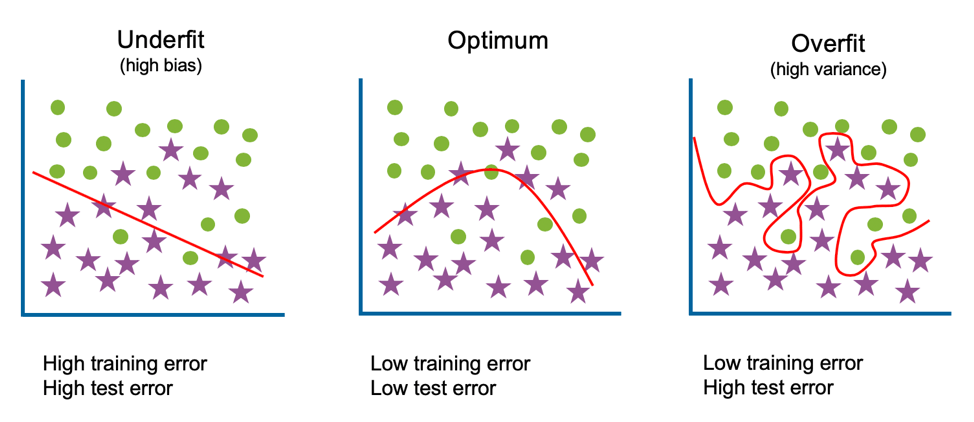
\includegraphics[scale=0.4]{model-over-fitting.png}
    \source{\autocite[]{ibm-overfitting:2022}}
    \caption{ Underfitting, optimal, overfitting machine learning model.}
\end{figure} 
A huge amount of dimensions also increases the computation costs and can reduce the performance in total. The more dimensions a data set has, the more prevalent it will contain redundant, noisy, and unimportant features, wich lead to overfitting and increase the error rate of the learning algorithm. Therefore, it can help to focus on a small subset of really important features. \autocite[]{CAI201870} \textcite[]{ALLAM2022329} \textcite[]{VenkateshAnuradha:2019} 
Feature selection is divided into two steps. The first step is to filter the data and reducing the feature space by removing the previously mentioned irrelevant features. In the second step, an optimal subset of features of the remaining data is created using a wrapper. \autocite[]{CAI201870}
This can be achieved by removing redundant and unimportant data columns to get enhance performance of prediction,  scalability  and  generalization  capability in learning efficiency and avoid overfitting. If a feature does not affect the prediction quality of the learning model, it is not important for the prediction \textcite[]{VenkateshAnuradha:2019}. This does not mean that this feature does not contain useful data. It only indicates that it is not statistically related to other features \textcite[]{VenkateshAnuradha:2019}.
 A good feature Selection can help to get much better predictions from the machine learning models and decrease the error rate \textcite[]{CAI201870}. 
In most feature selection methods, optimization algorithms are used to build a subset of the most relevant features. This leads to better performance and better classification results. \autocite[]{ALLAM2022329}
The popular approaches to do this, are models, features quality measures, feature evaluation, search strategies and combinations of these \textcite[]{VenkateshAnuradha:2019}.
Depending on how the training set is labeled, supervised (fully labeled), unsupervised (unlabeled) and semi-supervised (partially labeled) feature selection methods are used \textcite[]{CAI201870}.
Feature selection methods can also be divided into the three groups Filter, Wrapper and Embedded Method, based on how they interact on the learning models. \\
 The Filter method selects features based on statistical factors. It is used as part of preprocessing step in the feature selection, wich means this methods help to remove the not or less important features of a dataset before using the data to be fit on a classifier model. This method does not depend on the learning algorithms and therefore consumes much less time. For an Example there are correlation  coefficient or the chi-square test. \autocite[]{VenkateshAnuradha:2019} \textcite[]{CAI201870} \textcite[]{PISNER2020101} \\~\\
The Wrapper method totally depends on the classifier used, wich means it does need more computation time than the Filter method. On the other hand the best subset of features comes directly based on the results of the classifier and they are more accurate than the filter methods. \autocite[]{VenkateshAnuradha:2019} \textcite[]{CAI201870} These methods train the classifier repeatedly and validate the results of the model after each iteration. In this way, the quality of the feature subset is iteratively improved. Of course, depending on the classifier and data set, this approach can lead to large computation times, which should definitely be taken into account when using it. \autocite[]{PISNER2020101}
Wrapper models mostly use the accuracy rate and the classification error as default evaluation scores. The feature selection results of these models are often created at the same time as the results of the machine learning model. This is due to the fact that the learning model is embedded in the feature selection. \autocite[]{CAI201870}
An examples for this method are genetic algorithms. \\~\\
The third variant is the wrapper method. This performs better than the other two because it requires less computation time and makes collective decisions based on hybrid learning or ensemble learning. An example of such a method is the random forrest. \autocite[]{VenkateshAnuradha:2019} \textcite[]{CAI201870}
Feature selection methods should have a small time and space complexity and do not generate a lot of overhead, but must also have a high learning accuracy  \textcite[]{CAI201870}.
\\
\begin{figure}[h]
    \centering
    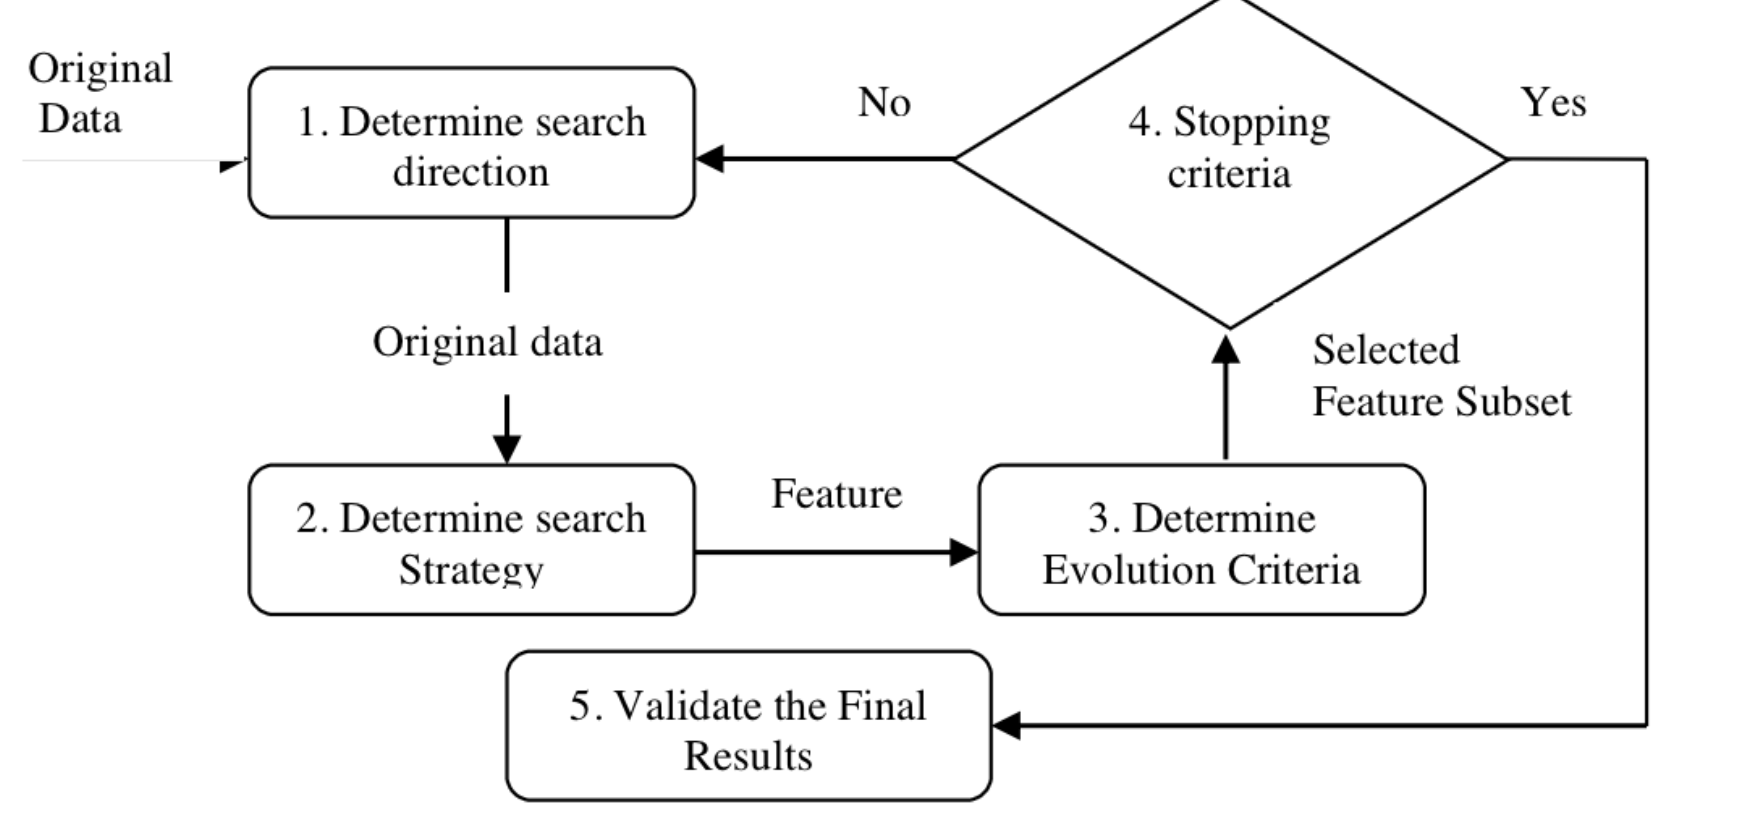
\includegraphics[scale=0.5]{FSprocess.png}
    \source{\autocite[]{VenkateshAnuradha:2019}}
    \caption{ Stages of the Feature Selection process.} 
\end{figure}
\\
Figure 2 shows the 5 steps of a feature selection process. The process starts by the search direction, wich can be forward, backward or random. The second step is to define wich of the three search strategies, randomized,  exponential  or  sequential, should be used. After that the feature selection method selects features by the use of the evaluation criteria. To reduce cost, computation time and complexity, it is important to specify a stopping criteria, wich leads to stop the process earlier, for example if there were no new improvements for a while. It defines the point on wich the method should break. \autocite[]{VenkateshAnuradha:2019}
For example the depth of a decision tree defines the maximum number of branches, nodes and leafs of the tree, wich also defines its maximum complexity.
After the feature selection algorithm finished it search process, the results must be validated. For this step there are a lot of methods. For example cross validation or confusion matrix. \autocite[]{VenkateshAnuradha:2019}
How important parameters were considered to be for the avalanches in each study seems to be strongly related to what parameters were available and wich machine learning models have been used for the study. 
As an example, in the study in Iran, wich is described in the article "Snow avalanche hazard prediction using machine learning methods" \textcite[]{Bahram:2019}, elevation was not ranked as particularly important for prediction, whereas in a study in India reported in the paper "Parameter importance assessment improves efficacy of machine learning methods for predicting snow avalanche sites in Leh-Manali Highway, India" \textcite[][]{Tiwari:2021}, it has been ranked as the second most important feature. 
In the First Study, more additional meteorological and geographic parameters were available, which appear to be more important than the elevation \textcite[]{Bahram:2019} \textcite[]{Tiwari:2021}.
Because of its low computation time for highly dimensional datasets and good results, in context of this thesis genetic algorithm is used as search strategy.  
In case of this thesis decision trees, logistic regression and SVM are used as classifiers for a Genetic Algorithm. The next three chapters describe these as well as the genetic algorithm in detail and give an understanding about how they are used to find the important features of an dataset. The Decision tree and Logistic regression models are also used to give an general understanding about statistical importance of all features in the dataset.


\subsubsection{Decision Tree}
The Decision tree is a powerful hierarchical supervised machine learning model wich is non-parametric and can be used for both, classification and regression problems. Additionally it is a recursive build data structure based on the concept of dividing-and-conquering \textcite[]{SUBASI202091}
 Or as it is defined in the documentation for the decision tree algorithm in the Python librars Scikit-learn: 
\begin{quote}
	"Decision Trees (DTs) are a non-parametric supervised learning method used for classification and regression. The goal is to create a model that predicts the value of a target variable by learning simple decision rules inferred from the data features. A tree can be seen as a piecewise constant approximation." \autocite{Scikit-learn-decision-tree:2022}
\end{quote}
These machine learning model is a representation method based on knowledge about the features of a dataset to represent classification rules \textcite[]{SUGUMARAN2007930}. 
Decision Trees use a set of if-than-else rules to decide wich value to predict. These models are good to understand, interpret and visualisable because they use white box models in wich every step is a boolean logic and easy explainable \textcite[]{Scikit-learn-decision-tree:2022}. For this reason, decision trees are also often preferred to other methods that actually provide accurate results \textcite[]{SUBASI202091}.
A standard decision tree starts with a root node, does have some branches as well as child nodes and leaves \textcite[]{SUGUMARAN2007930}. Each of these decision nodes labels the resulting nodes or leaves with discrete scores, wich shows how much the input set has been separated. The branch wich is chosen after each node depends on the input in combination with the test function of the node. \autocite[]{SUBASI202091} 
The root node splits the set by a rule on the features wich provides the best classification of the instance. This goes recursive till the max depth is reached or the classification is completed. So a branch is the path from the root node to the leaf. The leaf at the end of an branch, wich represent the class labels of the feature to predict. \autocite[]{SUGUMARAN2007930}
For the process of building a decision tree, the dataset is split into two or more subsets in each phase. For that in every phase it is searched for the best split for the input set. This process is continued recursively with the subsets until there is no need to split them anymore. This state can be reached by the tree it self, causing the fact that the resulting leaves are completely pure, or by the maximum depth stop criteria. This early stopping of the tree build is called prepruning, but there is also another method to simplify the tree called postpruning. This method grows the decision tree completely until all leaves are pure. Then all subtrees caused by overfitting are identified and pruned. This method can deliver better results in practice. \autocite[]{SUBASI202091}
It's also possible to use them to predict multiple values at the same time, wich is a typical problem in supervised machine learning called the Multi-output problem \textcite[]{Scikit-learn-decision-tree:2022}.
Decision Trees are likely to overfit if used on high dimensional datasets, but if used with a low tree depth, they can give a good understanding about the importance of some individual features for the prediction of multiple or specific parameters \textcite[]{Scikit-learn-decision-tree:2022}. The deeper the nodes are in the tree, the less important the features they represent are for the prediction. In addition, the decision tree contains only parameters that contribute to the prediction.
Therefore, not only the importance of the features for classification can be determined, but also whether they can be used for classification at all. \autocite[]{SUGUMARAN2007930}
This advantages of decision trees make them also useful for feature selection. 
In the case of the study, wich is represented in the article "Feature selection using Decision Tree and classification through Proximal Support Vector Machine for fault diagnostics of roller bearing" \textcite[]{SUGUMARAN2007930} Decision trees are used for the feature selection. Similar to this work, the study was concerned with a classification problem.




\subsubsection{Genetic algorithm}
Genetic algorithm is an evolutionary based adaptive optimization search methodology. They contain to the feature selection category of wrapper models. As a Wrapper it is used for the second step of feature selection to find an optimal subset of features for the learning algorithm \textcite[]{CAI201870}. Like a lot of other technical inventions, the functionality of genetic algorithms is inspired by nature. For example Neuronal Networks are inspired by the functionality of the human brain. Genetic algorithms resemble the Darwinian natural selection and evolution of species. They use this mechanisms to optimize modeling problems and get a good subset of features. Genetic algorithms simulate the natural selection of species \textcite[]{LU2008887} . This means only the species who survive environmental changes can become another generation. Each generation represents a population of individuals. Each of this individuals represents a single solution for the problem and is defined by a genetic string wich is build out of chromosomes wich represent encoded features. \autocite[]{LU2008887} \textcite[]{DBLP:1912}  Genteic algorithms are also able to handle huge dimensional datasets efficiently because of their exploitational and explorational characteristics \textcite[]{LU2008887}. The algorithm starts by creating a random generated population, wich happens by generating a number of chromosomes. After that step a classification model is constructed based on the combination of variables of each chromosome. This classification model is validated, on each chromosome, with an k-fold cross validation by the use of statistical scores like the accuracy score. The fitter chromosomes have a higher chance to get passed on to the next generation. After that the genetic algorithm selects and recombinates the chromosomes by the validation of the scores from parent and offspring to get a new population. It depends on the stop criteria whether the algorithm stops or runs the same cycle again with the new population. The algorithm needs an stopping criteria on wich it will stop processing new generations. \autocite[]{DBLP:1912} \textcite[]{Yang:2018} \textcite[]{LU2008887}\\
Jianjiang Lu and Tianzhong Zhao and Yafei Zhang \textcite[]{LU2008887} describe the three main operations for the process of a Genetic search methodology, wich are selection, crossover and mutation operation, as follows. The selection operation searches for the strongest N individuals from the current population. These are used as parents for the next generation of individual solutions.
The crossover operation is spliced into three steps. At first it generates \(C_N^2\) pairs of combinations between all parent individuals. 
Secondly it generates the two numbers \(a(0 < a < m)\) and \(b(0 < b < m − a)\), in wich \(m\) represents the length of each chromosome, \(a\) indicates the start position of the crossover operation and \(b\) is the length of the crossover operation. 
For the last step, it is assumed for each parent pair \(C_1^t = \{w_k\}\) and \(C_2^t = \{w_k'\}\) with \( k = a + 1, …\), where \(a + b \) are two gen groups. To generate two new individuals for the pool of individuals, wich is used in the mutation operation to generate a new population, the gens in the range of \([(a + 1), (a + b)]\)are exchanged. The exchange is carried out on the basis of the crossover rate \(P_c\) as follows \textcite[]{LU2008887}: \newline
\(C_1^t+1 = {w_1,k}, C_2^t+1 = {w_2,k} \), where \(w_1,k = \gamma * w_k' + (1 - \gamma) * w_k, w_2k = \gamma * w_k + (1 - \gamma) * w_k' \), in this context \(\gamma \) is a predefined constant.
The Mutation operation takes the, in the separation operation, created individuals into a pool with the parent individuals so that the variation in the new population is guaranteed. The \(K\) worst individuals out of this pool get a small mutation rate \(P_m\). After that a number of genes are pickt, from every individual, by the mutation operation and a new offspring is generated as following: when a gene \(w_k(w_k \in [0,1] \) is mutated and its next generation is\(w_k'\), the mutation operation is \textcite[]{LU2008887}: \\~\\
\( w_k' =
  \begin{cases}
    w_k + \Delta(t, 1 - w_k), & \eta = 0\\
    w_k + \Delta(t, w_k), & \eta = 1 
  \end{cases}
 \) \hfill \textcite[]{LU2008887} \\~\\~\\
 The variable \(\eta\) is a random number wich can be ether '1' or '0' and the return value of the function \(\Delta(t, \gamma)\) is in range \([0, \gamma]\) \textcite[]{LU2008887}.\\~\\
\(\Delta(t, \gamma) = \gamma (1 - r^{(1-\frac{t}{M})})\) \hfill \textcite[]{LU2008887} \\~\\
\(r\) is a number wich is randomly chosen in the range of \([0,1]\). Furthermore, \(t\) shows the value of the iterations. \(M\) represents the maximum of iterations and \(p\) indicates the predefined mutation parameter. Caused of this functions, the genetic algorithm mutates in earlier generations more than in later ones. \autocite[]{LU2008887} \newline
In the article "Grid Search, Random Search, Genetic Algorithm: {A} Big Comparison for {NAS}", Petro Liashchynskyi and Pavlo Liashchynskyi tested Grid Search, Random Search and Genetic Algorithm on the CIFAR-10 Dataset. They concluded that the Genetic algorithm took more time, but also produced better results. With larger numbers of features, it was even faster than the other two. \autocite[]{DBLP:1912}
The authors of the article "Predictor selection method for the construction of support vector machine (SVM)-based typhoon rainfall forecasting models using a non-dominated sorting genetic algorithm" \textcite[]{Yang:2018} used the genetic algorithm in combination with the SVM classifier for the prediction of typhoons. This natural disasters are dependent, as well as snow avalanches, on meteorological and topographical data. 

In the context of this thesis the genetic algorithm implementation GAFeatureSelectionCV contained in the sklearn-genetic-opt Python library \textcite{Sklearn_genetic_feature_docu:2022} is used.














\end{document}